% 2002 年上海理科第 13 题：复平面阴影区域
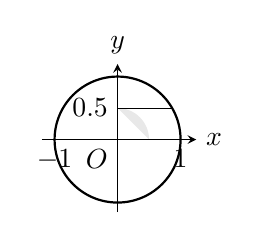
\begin{tikzpicture}[scale=0.8, >=stealth]
  \fill[gray!18] (0,0.5) arc (90:0:0.5) -- (0,0.5) -- cycle;
  \draw[thick] (0,0) circle (1);
  \draw[->] (-1.2,0)--(1.25,0) node[right] {$x$};
  \draw[->] (0,-1.15)--(0,1.2) node[above] {$y$};
  \draw (0,0.5)--(0.866,0.5);
  \node[left] at (0,0.5) {$0.5$};
  \node[below left] at (0,0) {$O$};
  \node[below] at (-1,0) {$-1$};
  \node[below] at (1,0) {$1$};
\end{tikzpicture}
